\subsection{Polyhedral code generation}\label{sec:affine}

One of the original motivations for \MLIR was the exploration of
polyhedral code generation for accelerators.
The affine dialect is a simplified polyhedral representation that was
designed to enable progressive lowering.
While a full exploration of the design points here is out of scope for this
paper, we illustrate aspects of the affine dialect to show the modeling power
of \MLIR and contrast the affine dialect with past
representations~\cite{Fea92b,uruk,isl,ppcg,tc}.

\subsubsection{Similarities}
The \MLIR affine dialect operates on a structured multi-dimensional
type for all accesses to memory.  In the default case, these structured types
are \emph{injective}: different indexings are guaranteed not to alias by
construction, a common precondition for polyhedral dependence analyses.

Affine modeling is split in two parts. Attributes are used to model affine
maps and integer sets at compile-time and Ops are used to apply affine
restrictions to the code. Namely, \lstinline|affine.for| Op is a ``for'' loop
with bounds expressed as affine maps of values required to be invariant in a
function. Thus loops have static control flow. Similarly,
\lstinline|affine.if| is a conditional restricted by affine integer sets.  The
bodies of loops and conditionals are regions that use \lstinline|affine.load|
and \lstinline|affine.store| to restrict indexing to affine forms of
surrounding loop iterators. This enables exact affine dependence analysis while
avoiding the need to infer affine forms from a lossy lower-level representation.

\begin{figure}[t]
  \centering
  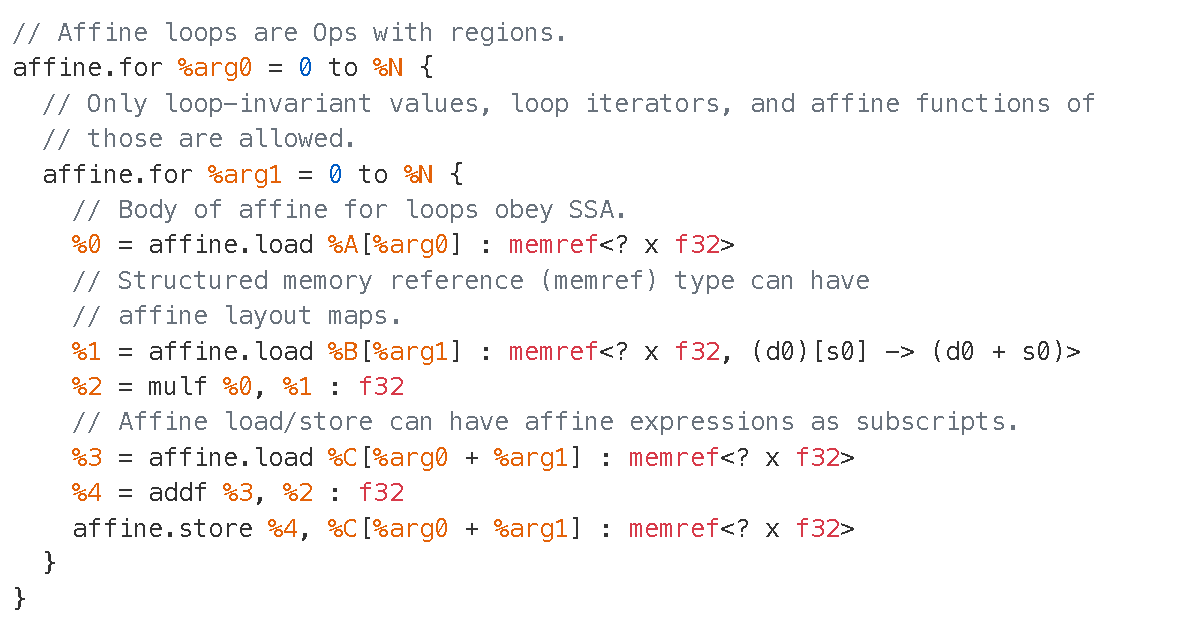
\includegraphics[width=.8\textwidth]{img/affine_mlir.pdf}
%  \lstinputlisting[language=mlir]{affine.mlir}
  \caption{Representing polynomial multiplication kernel
    \lstinline|C(i+j) += A(i) * B(j)| using \MLIR affine dialect.}
  \label{fig:affine}
\end{figure}

\subsubsection{Differences}
The differences with existing polyhedral frameworks are numerous, we can
characterize them in four categories:

(1) \emph{Rich types}: the \MLIR structured memory reference type contains a layout
map connecting the index space of the buffer to the actual address space.
This separation of concerns makes loop and data transformations compose better:
changes to data layout do not affect the code and do not pollute dependence
analysis. Such mixes of transformations have been explored
previously~\cite{chandan} but are uncommon.

(2) \emph{Mix of abstractions}: Bodies of affine loops in \MLIR can be expressed with
operations on typed SSA values.
Therefore, all traditional compiler analyses and transformations
remain applicable and can be interleaved with polyhedral transformations.  On
the contrary, polyhedral compilers often abstract such details away completely,
making it challenging for a polyhedral compiler to manipulate, e.g., vector
types.

(3) \emph{Smaller representation gap}: One of the key features of the polyhedral
model is its ability to represent the
order of loop iterations in the \emph{type system}. In this system, a large
number of loop transformations compose directly and can be reasoned about using
simple mathematical abstractions~\cite{uruk}. However, polyhedral
transformations require \emph{raising} into a representation often
drastically different from the original~\cite{polly,pollytactics}. Furthermore,
the conversion from
transformed polyhedra to loops is computationally hard~\cite{cloog}.
\MLIR-based representation maintains high-level loop structure around
lower-level representation, removing the need for raising.

(4) Compilation speed is a crucial goal for \MLIR as discussed in
\secref{parallel_comp}, but has not been a focus of most existing polyhedral
approaches.  These rely heavily on algorithms with exponential complexity: on integer
linear programming to derive loop orderings automatically and on polyhedron
scanning algorithms to convert the representation back to loops.
The approach taken by \MLIR explicitly does not rely on polyhedron scanning
since loops are preserved in the IR.

Experience with the affine dialect shows that it is useful for a wide range
of code generation projects, and its development was important exploration
that the \MLIR design made practical.

\iffalse
 A direct
consequence is that affine constructs are modeled as operations with special
semantics as described in 
\az{@ntv this must be finished}

Let us discuss several polyhedral representations. First algorithms by
Feautrier used multi-dimensional affine functions to express iteration
order~\cite{Fea92b}. The URUK framework separated the ordering between
individual loop iterations from the statement and loop ordering, which enabled
more declarative description of transformations and exploited the syntactic
structure to reduce the complexity of code generation~\cite{urgent}. Schedule
tree representation was driven by the GPU code generation needs
\az{cite Tobias Toplas}
and captures syntax-level ordering in an explicit tree structure
\az{cite Sven Impact}.
One can observe a trend towards including more of traditional compiler concepts
into polyhedral representations, partially attributable to the need for
mainstream adoption for polyhedral techniques.

\MLIR takes this integration further using the actual IR structure to represent
structural concepts, such as loop as branches, and by keeping most information
at the SSA value level, i.e. lifting everything into the type system.

\az{We need an actual description of how we encode polyhedral using IR
concepts, preferably before the discussion because the paper is about encoding
representations.}
For instance, the `affine.for` loop is still a higher-level type than
control-flow over basic blocks and generic `for` loops but does not have a
notion of iteration order. An `affine.for` loop produces an SSA-value for its
induction variable, that becomes a basic-block argument to the nested region.

\az{Etc describe affine in \MLIR, lift some example/desc from doc.}


%\subsubsection{Affine transformations}
%\TODO{do we want this?}
%
%\begin{figure}
%    \centering
%    %%\includegraphics{}
%    \caption{SGEMM performance comparison between code generated from affine dialect vs existing solutions.}
%    \label{fig:sgemm-results}
%\end{figure}

\fi
